\documentclass[xcolor=pdflatex,dvipsnames,table]{beamer}
\usepackage{epsfig,graphicx}
\usepackage{palatino}
\usepackage{fancybox}
\usepackage{relsize}
\usepackage[procnames]{listings}
\usepackage{hyperref}
\usepackage{qtree} % needed?
\usepackage{booktabs}
\usepackage{dirtree}
\usepackage[normalem]{ulem}


% fatter TT font
\renewcommand*\ttdefault{txtt}
% another TT, suggested by Alex
% \usepackage{inconsolata}
% \usepackage[T1]{fontenc} % needed as well?


\newcommand{\scale}{0.7}

\newcommand{\todo}[1]{{\emph{TODO: #1}}}
\newcommand{\martin}[1]{{\color{blue} Martin: #1}}
\newcommand{\abcdef}[1]{{\color{red} Author2: #1}}

% uncomment following for final submission
%\renewcommand{\todo}[1]{}
%\renewcommand{\martin}[1]{}
%\renewcommand{\author2}[1]{}

\newcommand{\code}[1]{{\texttt{#1}}}

\hypersetup{
  linkcolor  = black,
%  citecolor  = blue,
  urlcolor   = blue,
  colorlinks = true,
}

\beamertemplatenavigationsymbolsempty
\setbeamertemplate{footline}[frame number]





\newif\ifbook
% shared in slides and book

\lstdefinelanguage{chisel}{
  morekeywords={abstract,case,catch,class,def,%
    do,else,extends,false,final,finally,%
    for,if,implicit,import,match,mixin,%
    new,null,object,override,package,%
    private,protected,requires,return,sealed,%
    super,this,throw,trait,true,try,%
    type,val,var,while,with,yield},
  otherkeywords={=>,<-,<\%,<:,>:,\#,@},
  sensitive=true,
  morecomment=[l]{//},
  morecomment=[n]{/*}{*/},
  morestring=[b]",
  morestring=[b]',
  morestring=[b]"""
}

\usepackage{color}
\definecolor{dkgreen}{rgb}{0,0.6,0}
\definecolor{gray}{rgb}{0.5,0.5,0.5}
\definecolor{mauve}{rgb}{0.58,0,0.82}

% Default settings for code listings
\ifbook
\lstset{%frame=lines,
  language=chisel,
  aboveskip=3mm,
  belowskip=3mm,
  showstringspaces=false,
  columns=fixed, % basewidth=\mybasewidth,
  basicstyle={\small\ttfamily},
  numbers=none,
  numberstyle=\footnotesize,
  % identifierstyle=\color{red},
  breaklines=true,
  breakatwhitespace=true,
  procnamekeys={def, val, var, class, trait, object, extends},
  % procnamestyle=\ttfamily,
  tabsize=2,
  float
}
\else
\lstset{%frame=lines,
  language=chisel,
  aboveskip=3mm,
  belowskip=3mm,
  showstringspaces=false,
  columns=fixed, % basewidth=\mybasewidth,
  basicstyle={\small\ttfamily},
  numbers=none,
  numberstyle=\footnotesize\color{gray},
  % identifierstyle=\color{red},
  keywordstyle=\color{blue},
  commentstyle=\color{dkgreen},
  stringstyle=\color{mauve},
  breaklines=true,
  breakatwhitespace=true,
  procnamekeys={def, val, var, class, trait, object, extends},
  procnamestyle=\ttfamily\color{red},
  tabsize=2,
  float
}
\fi

\lstnewenvironment{chisel}[1][]
{\lstset{language=chisel,#1}}
{}

\newcommand{\shortlist}[1]{{\lstinputlisting[nolol]{#1}}}

\newcommand{\longlist}[3]{{\lstinputlisting[float, caption={#2}, label={#3}, frame=tb, captionpos=b]{#1}}}

\newcommand{\verylonglist}[3]{{\lstinputlisting[caption={#2}, label={#3}, frame=tb, captionpos=b]{#1}}}



\title{Components and Sequential Circuits}
\author{Martin Schoeberl}
\date{\today}
\institute{Technical University of Denmark\\
Embedded Systems Engineering}

\begin{document}

\begin{frame}
\titlepage
\end{frame}


\begin{frame}[fragile]{Overview}
\begin{itemize}
\item Start with bundle, IO, Moduls, main, App
\item Chisel: 3.1, 3.2, 4 and 6 (6.2., 6.3)
\item TODOs
\item have asX here and in the book
\item go through the book
\item Have a ref to the Java lecture
\item The main program (compare Java with Scala)
\item If time allows, repeat main points from timing lecture
\item A least have the Chisel code for the two flip-flop input synchronizer
\item Show git commands, in slides and do live the clone, update, and pull. Point to gui version. Show that you can even do the git pull in IntelliJ
\end{itemize}
\end{frame}

\begin{frame}[fragile]{Overview}
\begin{itemize}
\item Vending machine project
\item Repeat combinational building blocks
\item Power user II
\item Components and top-level
\item Sequential circuits
\item Chisel/VHLD comparison
\end{itemize}
\end{frame}


\begin{frame}[fragile]{Admin}
\begin{itemize}
\item How is the lab work going so far?
\item Start to organize yourself in groups of 2--3
\begin{itemize}
\item You can ask for finding a group via slack
\end{itemize}
\item Register at \href{https://docs.google.com/spreadsheets/d/1Hp81EyFYYvjm336DrwtCym9oRQUEzRKe6VceFp0ZCAQ/edit?usp=sharing}{Google spreadsheet}
\end{itemize}
\end{frame}


\begin{frame}[fragile]{A Vending Machine from 1952}
\begin{figure}
    \centering
    \href{https://en.wikipedia.org/wiki/File:CandiesVendingMachine1952.jpg}{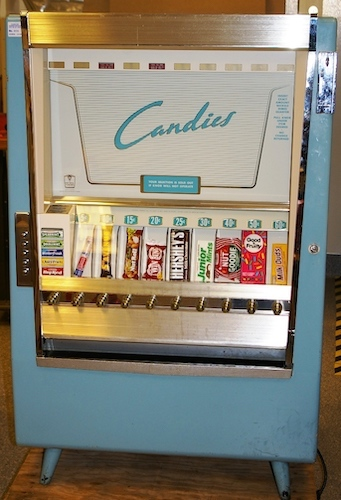
\includegraphics[scale=0.4]{CandiesVendingMachine1952}}

\end{figure}

{\tiny Source: Minnesota Historical Society, \href{https://creativecommons.org/licenses/by-sa/2.0}{CC BY-SA 2.0}}
\end{frame}

\begin{frame}[fragile]{The Vending Machine}
\begin{itemize}
\item Final project is a vending machine
\item \emph{Specification document is in DTU Inside (show it)}
\item Inputs: coins, buy
\item Display: price and current amount
\item Output: release can or error
\item Small challenge to multiplex the display
\item State machine with data path is the \emph{brain} of the VM
\item Guided step by step over several weeks
\end{itemize}
\end{frame}

\begin{frame}[fragile]{Vending Machine Specification I}
\begin{itemize}
\item Sell 1 item and not returning any money
\item Set price with 5 switches (1--31 kr.)
\item Display price on two 7-segment displays (hex.)
\item Accept 2 ad 5 kr. (two push buttons)
\item Display sum on two 7-segment displays (hex.)
\begin{itemize}
\item Amount entered so far
\end{itemize}
\item Does not return money, left for the next purchase
\end{itemize}
\end{frame}

\begin{frame}[fragile]{Vending Machine Specification II}
\begin{itemize}
\item Push button \emph{Buy}
\begin{itemize}
\item If not enough money, activate \emph{alarm} as long as buy is pressed
\item If enough money, activate \emph{release item} for as long as \emph{buy}
is pressed and reduce \emph{sum} by the price of the item
\end{itemize}
\item Optional extras (for a 12)
\begin{itemize}
\item Display decimal numbers
\item Supplement alarm by some visuals (e.g., blinking display)
\item Count coins and display an alarm when compartment is full ($>$ 20 coins)
\item Have some text scrolling on the display
\item ...
\item Your ideas :-)
\end{itemize}
\end{itemize}
\end{frame}

\begin{frame}[fragile]{Design and Implementation}
\begin{itemize}
\item Implementation shall be a state machine plus datapath
\item Design your datapath on a sheet of paper
\item Datapath
\begin{itemize}
\item Does add and subtract
\item Contains a register to hold the sum
\item Needs some mulitplexer to operate
\end{itemize}
\item Display needs multiplexing
\begin{itemize}
\item Implemented with some counters and a multiplexer
\end{itemize}
\item Show each part of your design to a TA
\begin{itemize}
\item 7-segment decoder, 7-segment with a counter, display multiplexer, complete vending machine
\end{itemize}
\end{itemize}
\end{frame}

\begin{frame}[fragile]{Vending Machine Design and Implementation Steps}
\begin{itemize}
\item We start next week
\item 2 + 2 + 3 + 3 + 4 + 4 = 18 supervised lab hours
\item 1a. Hexadecimal to 7-segment decoder
\item 1b. 7-segment display with a counter
\item 2. Multiplexed Seven-Segment Display
\item 3. Complete Vending Machine
\item \emph{Show your working design to a TA}
\end{itemize}
\end{frame}

\begin{frame}[fragile]{Final Report}
\begin{itemize}
\item One report per group
\item A single PDF
\begin{itemize}
\item Your group number is part of the file name (e.g., group7.pdf)
\item Code as listing in an appendix (no .zip files)
\item Hand in in DTU Inside
\end{itemize}
\item Content
\begin{itemize}
\item Abstract
\item Preface (Who did what)
\end{itemize}
\begin{enumerate}
\item Introduction and Problem Formulation
\item Analysis and Design
\item Implementation
\item Testing
\item Results
\item Discussion
\item Conclusion
\end{enumerate}
\begin{itemize}
\item List of References
\item Appendix: Chisel code
\end{itemize}
\end{itemize}
\end{frame}

\begin{frame}[fragile]{Questions on Final Project?}
\end{frame}

\begin{frame}[fragile]{Combinational Circuit with Conditional Update}
\begin{itemize}
\item Value first needs to be wrapped into a \code{Wire}
\item Updates with the Chisel update operation \code{:=}
\item With \code{when} we can express a conditional update
\item The condition is an expression with a Boolean result
\item The resulting circuit is a multiplexer
\item The rule is that the last enabled assignment counts
\begin{itemize}
\item Here the order of statements has a meaning
\end{itemize}
\end{itemize}
\shortlist{../code/comb_wire2.txt}
\end{frame}

\begin{frame}[fragile]{Comparison}
\begin{itemize}
\item The usual operations (as in Java or C)
\begin{itemize}
\item Unusual equal and unequal operator symbols
\item To keep the original Sala operators usable for references
\end{itemize}
\item Operands are \code{UInt} and \code{SInt}
\item Operands can be \code{Bool} for equal and unequal
\item Result is \code{Bool}
\end{itemize}
\begin{chisel}
>, >=, <, <=
===, =/=
\end{chisel}
\end{frame}

\begin{frame}[fragile]{Boolean Logical Operations}
\begin{itemize}
\item Operands and result are \code{Bool}
\item Logical NOT, AND, and OR
\end{itemize}
\begin{chisel}
val notX = !x
val bothTrue = a && b
val orVal = x || y
\end{chisel}
\end{frame}

\begin{frame}[fragile]{The ``Else'' Branch}
\begin{itemize}
\item We can express a form of ``else''
\item Note the \code{.} in \code{.otherwise}
\end{itemize}
\shortlist{../code/comb_otherwise.txt}
\end{frame}



\begin{frame}[fragile]{A Chain of Conditions}
\begin{itemize}
\item To test for different conditions
\item Select with a priority order
\item The first expression that is true counts
\item The hardware is a chain of multiplexers
\end{itemize}
\begin{columns}
\column{0.5\textwidth}
\shortlist{../code/comb_elsewhen.txt}
\column{0.5\textwidth}
\begin{figure}
  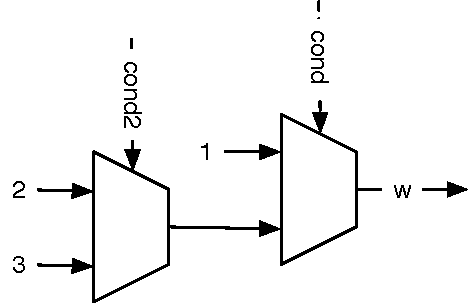
\includegraphics[scale=\scale]{../figures/mux-chain}
\end{figure}
\end{columns}
\end{frame}

\begin{frame}[fragile]{Default Assignment}
\begin{itemize}
\item Practical for complex expressions
\item Forgetting to assign a value on all conditions
\begin{itemize}
\item Would describe a latch
\item Runtime error in Chisel
\end{itemize}
\item Assign a default value is good practise
\end{itemize}
\shortlist{../code/comb_wiredefault.txt}
\end{frame}

\begin{frame}[fragile]{Logic Can Be Expressed as a Table}
\begin{itemize}
\item Sometimes more convenient 
\item Still combinational logic (gates)
\item Is converted to Boolean expressions
\item Let the synthesize tool do the conversion!
\item We use the \code{switch} statement
\end{itemize}
\shortlist{../code/encdec_decbin.txt}
\end{frame}


\begin{frame}[fragile]{A Decoder}
\begin{figure}
  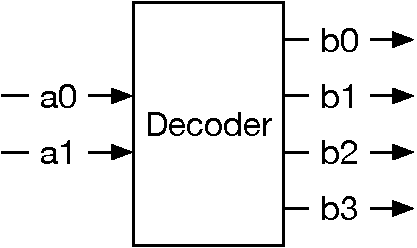
\includegraphics[scale=\scale]{../figures/decoder}
\end{figure}
\begin{itemize}
\item Converts a binary number of $n$ bits to an $m$-bit signal, where $m \leq 2^n$
\item The output is one-hot encoded (exactly one bit is one)
\item Building block for a $m$-way Mux
\item Used for address decoding in a computer system
\item Maybe of use for the display multiplexer
\end{itemize}
\end{frame}

\begin{frame}[fragile]{Truth Table of a Decoder}
\begin{table}
  \begin{tabular}{rr}
    \toprule
    a & b \\
    \midrule
    00 & 0001 \\
    01 & 0010 \\
    10 & 0100 \\
    11 & 1000 \\
    \bottomrule 
  \end{tabular} 
\end{table}
\end{frame}

\begin{frame}[fragile]{An Encoder}
\begin{figure}
  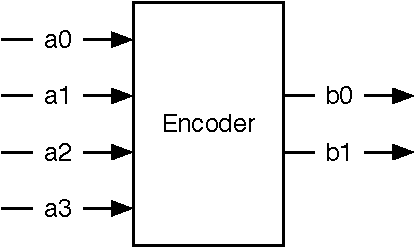
\includegraphics[scale=\scale]{../figures/encoder}
\end{figure}
\begin{itemize}
\item Converts one-hot encoded signal
\item To binary representation
\end{itemize}
\end{frame}

\begin{frame}[fragile]{Truth Table of an Encoder}
\begin{table}
  \begin{tabular}{rr}
    \toprule
    a & b \\
    \midrule
    0001 & 00 \\
    0010 & 01 \\
    0100 & 10 \\
    1000 & 11 \\
    ???? & ?? \\
    \bottomrule 
  \end{tabular} 
\end{table}
\begin{itemize}
\item Only defined for one-hot input
\end{itemize}
\end{frame}

\begin{frame}[fragile]{Encoder in Chisel}
\begin{itemize}
\item We cannot describe a function with undefined outputs
\item We use a default assignment of \code{"b00"}
\end{itemize}
\shortlist{../code/encdec_enc.txt}

\end{frame}



\begin{frame}[fragile]{Power User II}
\begin{itemize}
\item xxx
 * Talk about tools
   * see chapter 3 in pragmatic programmer
   * Tools amplify your talent. The better your tools, and the better you know how to use them, the more productive you can be.
   * Talk about google, man pages, or even plain --help
 * Use (and write) tools
 * link is missing: use simple bash scripts or Makefiles to remember commands (show examples)


 * Do power user in week 4
 * Have some slides, but mostly show demo
 * link to Linux intro
 * Use the Windows VM
 * open a powershell terminal
 * do a mkdir
 * do ls and cd
 * open browser to repo and copy string
 * do a git clone
 * cd and ls, maybe a cat
 * setup IntelliJ
 * run one exercise
 * switch to Mac and change minor thing
 * Do git commit/push
 * do a git pull in Windows, show in IntelliJ README.md
 * On Mac go to GitHub page
 * Do a change
 * On Windows do a git pull in IntelliJ
 * Say to take it easy, you do not need to do this, but it will help you to become a better engineer ;-)
\item \url{https://www.oreilly.com/learning/ten-steps-to-linux-survival}

\end{itemize}
\end{frame}

\begin{frame}[fragile]{Power User II}
\begin{itemize}
\item Every craftsmen starts with good-quality tools
\item ``Tools amplify your talent''\footnote{The Pragmatic Programmer: From Journeyman to Master, by Andrew Hunt and David Thomas}
\begin{itemize}
\item The better your tools, the more productive you are
\item The better you know them, the more productive you are
\end{itemize}
\item IDEs (Eclipse, InelliJ) are nice, I love them too
\item But we shall go beyond it
\item
\item
\item
\end{itemize}
\end{frame}

\begin{frame}[fragile]{Structure With Bundles}
\begin{itemize}
\item A \code{Bundle} to group signals
\item Can be different types
\item Defined by a class that extends \code{Bundle}
\item Named fields as \code{val}s within the block
\item Like a C struct or VHDL record
\end{itemize}
\shortlist{../code/bundle.txt}
\end{frame}

\begin{frame}[fragile]{Using a Bundle}
\begin{itemize}
\item Create it with \code{new}
\item Wrap it into a \code{Wire}
\item Field access with \emph{dot} notation
\end{itemize}
\shortlist{../code/bundle_use.txt}
\end{frame}



\begin{frame}[fragile]{Components}
\begin{itemize}
\item Components are building blocks
\item The have input and output ports (= pins)
\begin{itemize}
\item Organized as a \code{Bundle}
\end{itemize}
\item We build circuits as a hierarchy of components
\item In Chisel a component is called \code{Module}
\end{itemize}
\end{frame}

\begin{frame}[fragile]{Hierarchy of Components Example}
\begin{figure}
  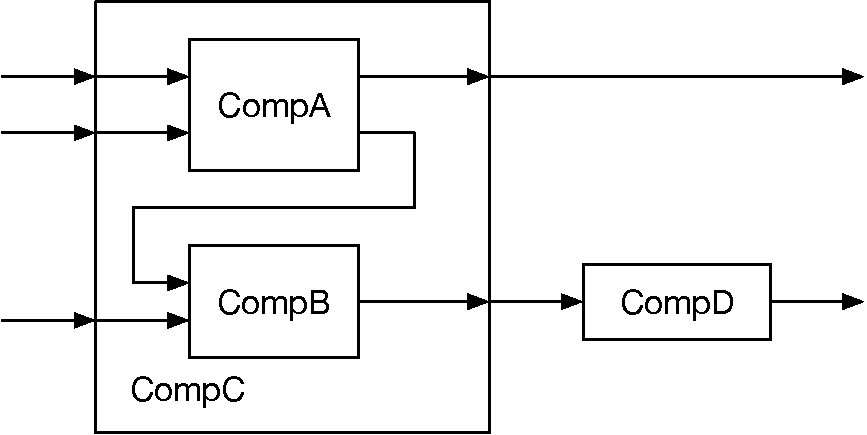
\includegraphics[scale=\scale]{../figures/components}
\end{figure}
\end{frame}

\begin{frame}[fragile]{Components CompA and CompB}
\shortlist{../code/components_ab.txt}
\end{frame}

\begin{frame}[fragile]{Component CompC}
\shortlist{../code/components_c.txt}
\end{frame}

\begin{frame}[fragile]{IO Ports}
\begin{chisel}
class Channel extends Bundle {
  val data = Input(UInt(8.W))
  val ready = Output(Bool())
  val valid = Input(Bool())
}
\end{chisel}
\begin{itemize}
\item Ports are Bundles with directions
\item Direction can also be assigned at instantiation:
\end{itemize}
\begin{chisel}
class ExecuteIO extends Bundle {
  val dec = Input(new DecodeExecute())
  val mem = Output(new ExecuteMemory())
}
\end{chisel}
\end{frame}

\begin{frame}[fragile]{Ports}
\begin{itemize}
\item Ports used to connect modules
\item Ports are bundles with directions
\end{itemize}
\begin{chisel}
class AluIO extends Bundle {
  val function = Input(UInt(2.W))
  val inputA = Input(UInt(4.W))
  val inputB = Input(UInt(4.W))
  val result = Output(UInt(4.W))
}
\end{chisel}
\end{frame}

\begin{frame}[fragile]{Port Directions}
\begin{itemize}
\item Can be reversed with the \code{Flipped}
\item Convenient to have one bundle definition working as source
and destination used between two modules
\end{itemize}
\begin{chisel}
class Channel extends Bundle {
  val data = Input(UInt(32.W))
  val ready = Output(Bool())
  val valid = Input(Bool())
}

class ChannelUsage extends Bundle {
  val input = new Channel()
  val output = Flipped(new Channel())
}
\end{chisel}
\end{frame}

\begin{frame}[fragile]{Port Directions}
\begin{itemize}
\item Can be assigned at instantiation
\end{itemize}
\begin{chisel}
class ExecuteIO extends Bundle {
  val dec = Input(new DecodeExecute())
  val mem = Output(new ExecuteMemory())
}
\end{chisel}
\begin{chisel}
\end{chisel}
\end{frame}


\begin{frame}[fragile]{Modules}
\begin{chisel}
class Adder extends Module {
  val io = IO(new Bundle {
    val a = Input(UInt(4.W))
    val b = Input(UInt(4.W))
    val result = Output(UInt(4.W))
  })

  val addVal = io.a + io.b
  io.result := addVal
}
\end{chisel}
\begin{itemize}
\item Organization of components
\item IO ports defined as a Bundle named \code{io} and wrapped into an \code{IO()}
\item Created (instantiated) with:
\end{itemize}
\begin{chisel}
val adder = Module(new Adder())
\end{chisel}
\end{frame}

\begin{frame}[fragile]{Connections}
\begin{itemize}
\item Simple connections just with assignments, e.g.,
\begin{chisel}
  adder.io.a := ina
  adder.io.b := inb
\end{chisel}
\item Automatic bulk connections between components
\begin{chisel}
  dec.io <> exe.io
  mem.io <> exe.io
\end{chisel}
\end{itemize}
\end{frame}






\begin{frame}[fragile]{Modules}
\begin{itemize}
\item Modules are used to organize the circuit
\item Similar to VHDL components (entity/architecture)
\item A class that inherits from \code{Module}
\item Circuit description in the constructor
\item Interface (port) is a \code{Bundle}, wrapped into an \code{IO()}, and stored in the field \code{io}
\end{itemize}
\begin{chisel}
class Adder extends Module {
  val io = IO(new Bundle {
    val a = Input(UInt(4.W))
    val b = Input(UInt(4.W))
    val result = Output(UInt(4.W))
  })

  val addVal = io.a + io.b
  io.result := addVal
}
\end{chisel}
\end{frame}

\begin{frame}[fragile]{Module Usage}
\begin{itemize}
\item Create with \code{new} and wrap into a \code{Module()}
\item Interface port via the \code{io} field
\item Note the assignment operator \code{:=} on \code{io} fields
\end{itemize}
\begin{chisel}
  val adder = Module(new Adder())
  adder.io.a := ina
  adder.io.b := inb
  val result = adder.io.result
\end{chisel}
\end{frame}


\begin{frame}[fragile]{Chisel Main}

\begin{itemize}
\item Create one top-level Module
\item Invoke the Chisel driver from the Scala \code{main} (or App)
\item Pass some parameters and the top module
\item Following code generates Verilog code
\end{itemize}
\begin{chisel}
object Hello extends App {
  chisel3.Driver.execute(Array[String](), () => new Hello())
}
\end{chisel}
\end{frame}


\begin{frame}[fragile]{XXX}
\begin{itemize}
\item
\item
\item
\end{itemize}
\end{frame}

\begin{frame}[fragile]{Verilog Generation}
\begin{itemize}
\item TODO: show individual snippets
\item on @[Hello.scala 17:23]
\begin{itemize}
\item
\end{itemize}
\item about pin names, e.g., \code{io\_led}
\item
\item
\item
\item
\end{itemize}
\begin{verbatim}
module Hello(
  input   clock,
  input   reset,
  output  io_led
);
  reg [31:0] cntReg; // @[Hello.scala 17:23]
  reg [31:0] _RAND_0;
  reg  blkReg; // @[Hello.scala 18:23]
  reg [31:0] _RAND_1;
  wire [31:0] _T_1; // @[Hello.scala 20:20]
  wire  _T_2; // @[Hello.scala 21:15]
  wire  _T_3; // @[Hello.scala 23:15]
  assign _T_1 = cntReg + 32'h1; // @[Hello.scala 20:20]
  assign _T_2 = cntReg == 32'h2faf07f; // @[Hello.scala 21:15]
  assign _T_3 = ~ blkReg; // @[Hello.scala 23:15]
  assign io_led = blkReg; // @[Hello.scala 25:10]
`ifdef RANDOMIZE_GARBAGE_ASSIGN
`define RANDOMIZE
`endif
`ifdef RANDOMIZE_INVALID_ASSIGN
`define RANDOMIZE
`endif
`ifdef RANDOMIZE_REG_INIT
`define RANDOMIZE
`endif
`ifdef RANDOMIZE_MEM_INIT
`define RANDOMIZE
`endif
`ifndef RANDOM
`define RANDOM $random
`endif
`ifdef RANDOMIZE_MEM_INIT
  integer initvar;
`endif
`ifndef SYNTHESIS
initial begin
  `ifdef RANDOMIZE
    `ifdef INIT_RANDOM
      `INIT_RANDOM
    `endif
    `ifndef VERILATOR
      `ifdef RANDOMIZE_DELAY
        #`RANDOMIZE_DELAY begin end
      `else
        #0.002 begin end
      `endif
    `endif
  `ifdef RANDOMIZE_REG_INIT
  _RAND_0 = {1{`RANDOM}};
  cntReg = _RAND_0[31:0];
  `endif // RANDOMIZE_REG_INIT
  `ifdef RANDOMIZE_REG_INIT
  _RAND_1 = {1{`RANDOM}};
  blkReg = _RAND_1[0:0];
  `endif // RANDOMIZE_REG_INIT
  `endif // RANDOMIZE
end // initial
`endif // SYNTHESIS
  always @(posedge clock) begin
    if (reset) begin
      cntReg <= 32'h0;
    end else if (_T_2) begin
      cntReg <= 32'h0;
    end else begin
      cntReg <= _T_1;
    end
    if (reset) begin
      blkReg <= 1'h0;
    end else if (_T_2) begin
      blkReg <= _T_3;
    end
  end
endmodule

\end{verbatim}
\end{frame}

\begin{frame}[fragile]{File Organization in Scala/Chisel}
\begin{itemize}
\item A Scala file can contain several classes (and objects)
\item For large classes use one file per class with the class name
\item Scala has packages, like Java
\item Use folders with the package names for file organization
\item \code{sbt} looks into current folder and \code{src/main/scala/}
\item Tests shall be in \code{src/test/scala/}
\end{itemize}
\end{frame}

\begin{frame}[fragile]{File Organization in Scala/Chisel}
\dirtree{%
.1 project.
.2 src.
.3 main.
.4 scala.
.5 package.
.6 sub-package.
.3 test.
.4 scala.
.5 package.
.2 target.
.2 generated.
}
\end{frame}


\begin{frame}[fragile]{Register (Again)}
\begin{itemize}
\item Sequential building blocks
\begin{itemize}
\item Contain a register
\item Plus combinational circuits
\end{itemize}
\end{itemize}
\begin{figure}
  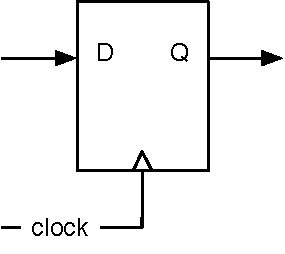
\includegraphics[scale=\scale]{../figures/register}
\end{figure}
\shortlist{../code/sequ_reg.txt}
\end{frame}



\begin{frame}[fragile]{Register in Two Steps}
\shortlist{../code/sequ_reg2.txt}
\end{frame}

\begin{frame}[fragile]{Register With Reset}
\begin{figure}
  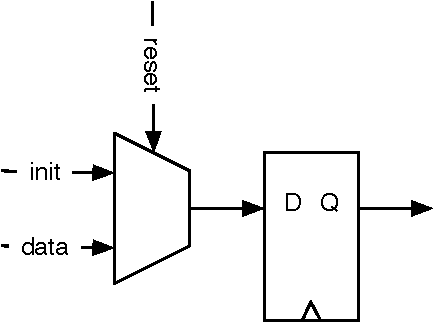
\includegraphics[scale=\scale]{../figures/register-reset}
\end{figure}
\shortlist{../code/sequ_reg_init.txt}
\end{frame}

\begin{frame}[fragile]{Timing Diagram of the Register with Reset}
\begin{figure}
  \includegraphics[scale=1]{../figures/reg_wave}
\end{figure}
\begin{itemize}
\item Also called waveform diagram
\item Logic function over time
\item Can be used to describe a circuit function
\item Useful for debugging
\end{itemize}
\end{frame}

\begin{frame}[fragile]{Register with Enable}
\begin{figure}
  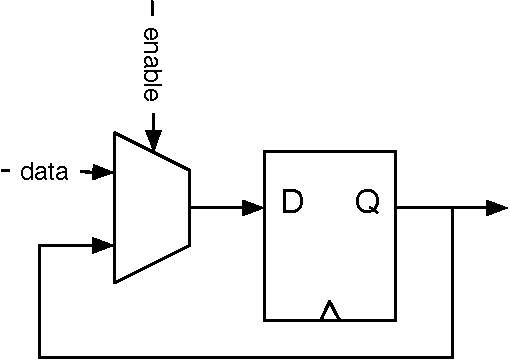
\includegraphics[scale=\scale]{../figures/register-enable}
\end{figure}
\begin{itemize}
\item Only when \code{enable} true is a value is stored
\end{itemize}
\shortlist{../code/sequ_reg_ena.txt}

\end{frame}

\begin{frame}[fragile]{Timing Diagram for an Enable Register}
\begin{figure}
  \includegraphics[scale=1]{../figures/reg_en_wave}
\end{figure}
\end{frame}

\begin{frame}[fragile]{More on Register}
\begin{itemize}
\item We can combine initialization and enable
\end{itemize}
\shortlist{../code/sequ_reg_init_ena.txt}
\begin{itemize}
\item A register can also be part of an expression
\item What does the following circuit do?
\end{itemize}
\shortlist{../code/sequ_reg_rising.txt}
\end{frame}


\begin{frame}[fragile]{Combine a Register with an Adder}
\begin{figure}
  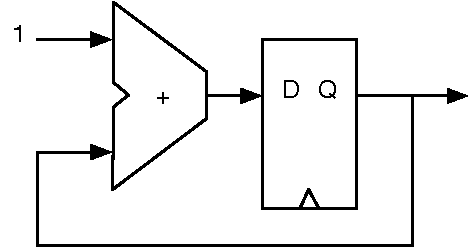
\includegraphics[scale=\scale]{../figures/counter}
\end{figure}
\begin{itemize}
\item Is a free running counter
\item 0, 1, ... 14, 15, 0, 1, ...
\end{itemize}
\shortlist{../code/sequ_free_counter.txt}
\end{frame}


\begin{frame}[fragile]{A Counter}
\shortlist{../code/counter.txt}
\begin{itemize}
\item This counter counts from 0 to 9
\item And starts from 0 again after reaching 9
\begin{itemize}
\item Starting from 0 is common in computer engineering
\end{itemize}
\item A counter is the hardware version of a \emph{for loop}
\item Often needed
\item Can you draw the schematic?
\end{itemize}
\end{frame}

\begin{frame}[fragile]{Counting Events}
\begin{figure}
  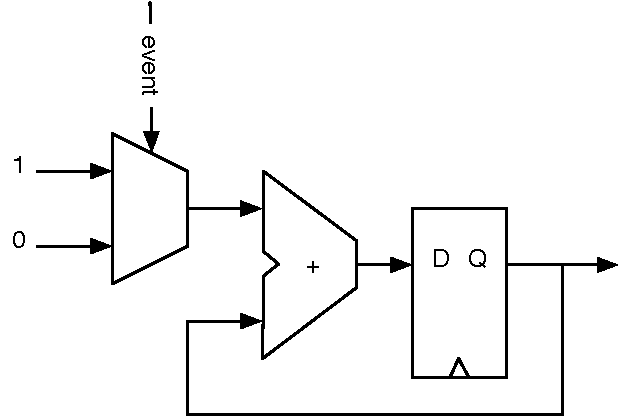
\includegraphics[scale=\scale]{../figures/event-counter}
\end{figure}
\begin{itemize}
\item Is the schematics and the code the same?
\end{itemize}
\shortlist{../code/sequ_event_counter.txt}
\end{frame}


\begin{frame}[fragile]{XXX}
\begin{itemize}
\item xxx
\begin{itemize}
\item
\end{itemize}
\item
\item
\item
\item
\item
\end{itemize}
\end{frame}



\begin{frame}[fragile]{XXX}
\begin{itemize}
\item xxx
\begin{itemize}
\item
\end{itemize}
\item
\item
\item
\item
\item
\end{itemize}
\end{frame}


\begin{frame}[fragile]{XXX}
\begin{itemize}
\item xxx
\begin{itemize}
\item
\end{itemize}
\item
\item
\item
\item
\item
\end{itemize}
\end{frame}

\begin{frame}[fragile]{Common Acronyms}
\begin{description}
\item [ADC] analog-to-digital converter
\item [ALU] arithmetic and logic unit
\item [ASIC] application-specific integrated circuit
\item [Chisel] constructing hardware in a Scala embedded language
\item [CISC] complex instruction set computer
\item [CRC] cyclic redundancy check
\item [DFF] D flip-flop, data flip-flop
\item [DMA] direct memory access
\item [DRAM] dynamic random access memory
\item [FF] flip-flop
\item [FIFO] first-in, first-out
\item [FPGA] field-programmable gate array
\item [HDL] hardware description language
\item [HLS] high-level synthesis
\item [IC] instruction count
\item [IDE] integrated development environment
\item [IO] input/output
\end{description}
\end{frame}

\begin{frame}[fragile]{Common Acronyms II}
\begin{description}
\item [ISA] instruction set architecture
\item [JDK] Java development kit
\item [JIT] just-Iin-time
\item [JVM] Java virtual machine
\item [LC] logic cell
\item [LRU] least-recently used
\item [MMIO] memory-mapped IO
\item [MUX] multiplexer
\item [OO] object oriented
\item [RISC] reduced instruction set computer
\item [SDRAM] synchronous DRAM
\item [SRAM] static random access memory
\item [TOS] top-of stack
\item [UART] universal asynchronous receiver/transmitter
\item [VHDL] VHSIC hardware description language
\item [VHSIC] very high speed integrated circuit
\end{description}
\end{frame}

\begin{frame}[fragile]{Chisel VHDL Comparison}
\begin{columns}
\column{0.5\textwidth}
\begin{chisel}
class DecodeExecute extends Bundle {
  val rs1 = UInt(32.W)
  val rs2 = UInt(32.W)
  val immVal = UInt(32.W)
  val aluOp = new AluOp()
}
\end{chisel}
\column{0.5\textwidth}
\begin{verbatim}
VHDL code here
\end{verbatim}
\end{columns}
Also show latch and and using a button as clock
\end{frame}

\begin{frame}[fragile]{Lab Today}
\begin{itemize}
\item Components and Small Sequential Circuits
\item \href{https://github.com/schoeberl/chisel-lab/tree/master/lab4}{Lab 4 Page}
\item You need to download again, as I have updated the lab
\begin{itemize}
\item Or learn to use git and do a  \code{git pull} ;-)
\end{itemize}
\item Each exercise contains a test, which initially fails
\item \code{sbt test} runs them all
\begin{itemize}
\item To just run a single test, run e.g.,\\
\code{sbt "testOnly SingleTest"}
\end{itemize}
When all test succeed your are done ;-)
\item Except: additional some drawing exercise
\end{itemize}
\end{frame}

\begin{frame}[fragile]{Summary}
\begin{itemize}
\item xxx
\item
\item
\item
\end{itemize}
\end{frame}

\begin{frame}[fragile]{Below Stuff from Tutorial}
\begin{itemize}
\item xxx
\item
\item
\item
\end{itemize}
\end{frame}






\begin{frame}[fragile]{Chisel and Scala}
\begin{itemize}
\item Chisel is a library written in Scala
\begin{itemize}
\item Import the library with \code{import chisel3.\_}
\end{itemize}
\item Chisel code is Scala code
\item When it is run is \emph{generates} hardware
\begin{itemize}
\item Verilog for synthesize
\item Scala netlist for simulation (testing)
\end{itemize}
\item Chisel is an embedded domain specific language
\item Two languages in one can be a little bit confusing
\end{itemize}
\end{frame}

\begin{frame}[fragile]{Scala}
\begin{itemize}
\item Is object oriented
\item Is functional
\item Strongly typed with very good type inference
\item Runs on the Java virtual machine
\item Can call Java libraries
\item Consider it as Java++
\begin{itemize}
\item Can almost be written like Java
\item With a more lightweight syntax
% \item Scala for Java Refugees is a nice tutorial (but link is dead)
% \item \url{http://www.codecommit.com/blog/scala/roundup-scala-for-java-refugees}
\end{itemize}
\end{itemize}
\end{frame}

\begin{frame}[fragile]{Scala Hello World}
\begin{chisel}
object HelloWorld extends App {
  println("Hello, World!")
}
\end{chisel}
\begin{itemize}
\item Compile with \code{scalac} and run with \code{scala}
\item You can even use Scala as scripting language
\item Show both
\end{itemize}
\end{frame}



\begin{frame}[fragile]{Generic Components}
\begin{chisel}
val c = Mux(cond, a, b)
\end{chisel}
\begin{itemize}
\item This is a multiplexer
\item Input can be any type
\end{itemize}
\end{frame}

\begin{frame}[fragile]{Testing}
\begin{chisel}
class CounterTester(c: Counter) extends PeekPokeTester(c) {
  for (i <- 0 until 5) {
    println(i.toString + ": " + peek(c.io.out).toString())
    step(1)
  }
}
\end{chisel}
\begin{itemize}
\item Within Chisel with a tester (= Scala program)
\item May include waveform generation
\item peek and poke to read and set values
\begin{itemize}
\item Remember the BASIC days ;-)
\end{itemize}
\item printf in simulation on rising edge
\begin{chisel}
printf("Counting %x\n", r1)
\end{chisel}
\end{itemize}
\end{frame}



\begin{frame}[fragile]{Scala Build Tool (sbt)}
\begin{itemize}
\item Downloads Scala compiler if needed
\item Downloads dependent libraries (e.g., Chisel)
\item Compiles Scala programs
\item Executes Scala programs
\item Does a lot of magic, maybe too much
\item Compile and run with:
\end{itemize}
\begin{chisel}
sbt "runMain simple.Example"
\end{chisel}
\begin{itemize}
\item Or even just:
\end{itemize}
\begin{chisel}
sbt run
\end{chisel}
\end{frame}

\begin{frame}[fragile]{Build Configuration}
\begin{itemize}
\item Defines needed Scala version
\item Library dependencies
\item File name: \code{build.sbt}
\end{itemize}
\begin{chisel}
scalaVersion := "2.11.7"

resolvers ++= Seq(
  Resolver.sonatypeRepo("snapshots"),
  Resolver.sonatypeRepo("releases")
)

libraryDependencies += "edu.berkeley.cs" %% "chisel3" % "3.1.2"
libraryDependencies += "edu.berkeley.cs" %% "chisel-iotesters" % "1.2.2"
\end{chisel}
\end{frame}


\begin{frame}[fragile]{What is a Minimal Chisel Project?}
\begin{itemize}
\item Scala class (e.g., \code{Hello.scala})
\item Build info in \code{build.sbt} for \code{sbt}:
\end{itemize}
\begin{chisel}
scalaVersion := "2.11.7"

libraryDependencies += "edu.berkeley.cs" %% "chisel3" % "3.1.2"
\end{chisel}
\begin{itemize}
\item Run the process manually (look into the Makefile)
\end{itemize}
\end{frame}




\begin{frame}[fragile]{Chisel Main for Testing}
\begin{itemize}
\item Tests can be written in Scala/Chisel
\item Tester and device under test (DUT) are two processes
\item Invoke \code{execute} with some parameters, the DUT, and a tester
\end{itemize}
\begin{chisel}
object CounterTester extends App {

  iotesters.Driver.execute(Array[String](), () => new Counter(2)) {
    c => new CounterTester(c)
  }
}
\end{chisel}
\end{frame}

\begin{frame}[fragile]{A Chisel Tester}
\begin{itemize}
\item Extends class \code{PeekPokeTester}
\item Has the DUT as parameter
\item Testing code can use all features of Scala
\end{itemize}
\begin{chisel}
class CounterTester(dut: Counter) extends PeekPokeTester(dut) {

  // Here comes the Chisel/Scala code
  // for the testing
}
\end{chisel}
\end{frame}

\begin{frame}[fragile]{Testing}
\begin{itemize}
\item Set input values with \code{poke}
\item Advance the simulation with \code{step}
\item Read the output values with \code{peek}
\item Compare the values with \code{expect}
\end{itemize}
\end{frame}

\begin{frame}[fragile]{Testing Example}
\begin{chisel}
// Set input values
poke(dut.io.a, 3)
poke(dut.io.b, 4)
// Execute one iteration
step(1)
// Print the result
val res = peek(dut.io.result)
println(res)

// Or compare against expected value
expect(dut.io.result, 7)
\end{chisel}
\end{frame}

\begin{frame}[fragile]{A Tiny ALU: IO Connection}
\begin{chisel}
class Alu extends Module {
  val io = IO(new Bundle {
    val fn = Input(UInt(2.W))
    val a = Input(UInt(4.W))
    val b = Input(UInt(4.W))
    val result = Output(UInt(4.W))
  })

  // Use shorter variable names
  val fn = io.fn
  val a = io.a
  val b = io.b
\end{chisel}
\end{frame}

\begin{frame}[fragile]{A Tiny ALU: The Function}
\begin{chisel}
  val result = Wire(UInt(4.W))
  // some default value is needed
  result := 0.U

  // The ALU selection
  switch(fn) {
    is(0.U) { result := a + b }
    is(1.U) { result := a - b }
    is(2.U) { result := a | b }
    is(3.U) { result := a & b }
  }

  // Output on the LEDs
  io.result := result
}
\end{chisel}
\end{frame}

\begin{frame}[fragile]{Testing the ALU}
\begin{itemize}
\item Compute the expected result in Scala
\end{itemize}
\begin{chisel}
  // This is exhaustive testing,
  // which usually is impossible
  for (a <- 0 to 15) {
    for (b <- 0 to 15) {
      for (op <- 0 to 3) {
        val result =
          op match {
            case 0 => a + b
            case 1 => a - b
            case 2 => a | b
            case 3 => a & b
          }
        val resMask = result & 0x0f
\end{chisel}

\end{frame}

\begin{frame}[fragile]{Testing the ALU}
\begin{itemize}
\item Compare the Scala computed result with the hardware result
\end{itemize}
\begin{chisel}
        poke(dut.io.fn, op)
        poke(dut.io.a, a)
        poke(dut.io.b, b)
        step(1)
        expect(dut.io.result, resMask)
      }
    }
  }
\end{chisel}
\end{frame}

\begin{frame}[fragile]{Generating Wave Forms}
\begin{itemize}
\item Additional parameters: \code{"--generate-vcd-output", "on"}
\item IO signals and registers are dumped
\item Option \code{--debug} puts all wires into the dump
\item Generates a .vcd file
\item Viewing with gtkwave or ModelSim
\item See the example with \code{make fifo}
\begin{itemize}
\item Show it
\end{itemize}
\item BubbleFifo contains also longer testing code
\end{itemize}
\end{frame}

\begin{frame}[fragile]{Summary}
\begin{itemize}
\item abc
\end{itemize}
\end{frame}


\end{document}
